\documentclass[14pt]{extarticle}
\usepackage{amsmath, amsfonts, amsthm, amssymb,graphicx}
\title{America vs. The World: A new Installation in the Thrilling Battle}
\author{Sridevi Suresh}

\setlength{\evensidemargin}{0.0in}
\setlength{\oddsidemargin}{0.0in}
\usepackage[footskip=0.25in]{geometry}
\setlength{\textwidth}{6in}

\begin{document}
\maketitle 

America: the land of the brave, the land of the free, the land of I'm-gonna-do-whatever-I-want. For years, Americans have been griping about how America is the best country in the world. While there are some good points as to why America is pretty star-spangling awesome, I still have a couple issues that I cannot get over. There is a growing list of idiosyncrasies that we see in America and not in \textit{any other country in the world}. 

At this point, you're probably thinking: "hey! Who is this girl trying to hate on 'murica?" Well, my dear reader, let me enlighten you on a couple facts.  Here is my growing list of things that make America different from the rest of the world:

\vspace{5mm}
1.) \textbf{The Metric System}. It's like America woke up one day and decided "oh you measure everything in kilograms? Okay, let me do all of my measurements in pounds just to confuse everyone ever." 

\vspace{5mm}
2.) \textbf{Gaps in public toilet doors.} Apparently, the rest of the world is shocked by the fact that all Americans want to be peeping Tom's. Did you know that visitors to the U.S are surprised when they see that we have inch-wide gaps around toilet stall doors? All other countries like to do their private business in just exactly that--private. 

\vspace{5mm}
3.) \textbf{Wearing shoes in the house.} Americans like to be dirty. Plain and simple. In most countries, you take your shoes off when entering someone's home. However, here in the good ole' land of the free, we just track whatever is underneath our shoes wherever we go. 

\vspace{5mm}
4.) \textbf{Telling time.} America uses a 12-hour clock with AM and PM, while the rest of the world uses a 24-hour clock. We just wanted time to be more confusing to the kids learning it for the first time. 

\vspace{5mm}
5.) \textbf{Automatic vs. Manual Transmission} Most of the world drives cars with manual transmission, but not America, no. We use automatic transmission because that just allows us to be more lazy. 

\vspace{5mm}
6.) \textbf{Football vs. soccer.} Do I even need to explain this one?

\vspace{5mm}
7.) \textbf{Corn syrup vs. sugar}. While America uses high fructose corn syrup as a sweetener, other countries in the world still use cane sugar. [Insert fat joke about America here]. 

\vspace{5mm}
8.) \textbf{PB\& J} Apparently, PB\& J is a true American delicacy. Other people in the world just don't get it. (Okay, I admit I love PB\& J but since I'm allergic to peanuts this goes on the list anyway). 

\vspace{5mm}
9.) \textbf{Eating pizza.} Okay, let's be real. Pizza is a staple food for most Americans and, more explicitly, broke college students. However, we eat our pizza the way it's supposed to be eaten while people from other countries eat it with a knife and fork. A knife and fork?! Didn't know the Queen of England was watching me eat my pizza...Maybe this should be off the list...

\vspace{5mm}
10.) \textbf{Americans are crazy about eggs.} Let's dive a little deeper into the topic of food, shall we? I decided to put my over-priced American college education to use. I used YY Ahn's data set \textit{Recipe datasets with cuisines} to do a  bit of hierarchical clustering to see if American cuisines truly do differ from other cuisines. I took the all\_recipes data and map data to creat a matrix where the rows are the different regions of the world and the columns are the different ingredients that appear in all the recipes. An entry in the matrix is a count of how many times that ingredient appears in a recipe that belongs to that specific region of the world. I, then, performed hierarchical clustering using the scipy library and have this visualization: 

\centering
\begin{minipage}[t]{.9\textwidth}
	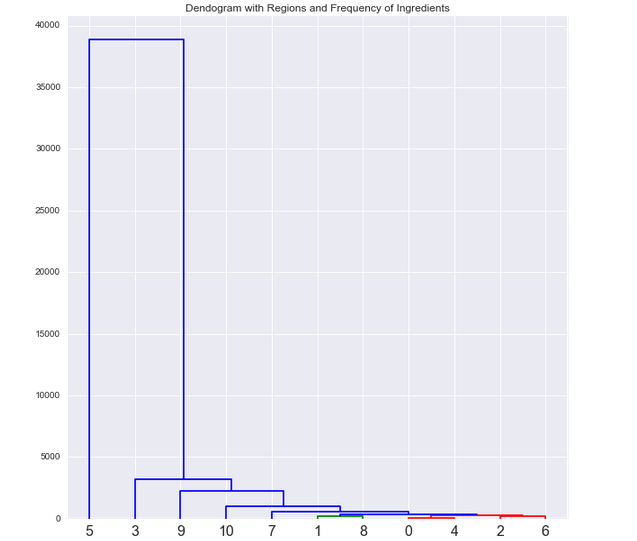
\includegraphics[width=\textwidth]{Regions_Ingredients.png}
\end{minipage}

\raggedright

Here, the 5 corresponds to North America and, thus, we see from this clustering that North American recipes are separated the most from recipes from other parts of the world. This made me curious and I decided to look further into North America and see what country's cuisine it is that is the most different from the rest of the wold. Spoiler alert: it's America. 

This time I just used the all\_recipes data to create a similar matrix as above, except this time the rows correspond to a country cuisine. Again, performing hierarchical clustering using scipy, I get the following visualization:

\centering
\begin{minipage}[t]{.9\textwidth}
	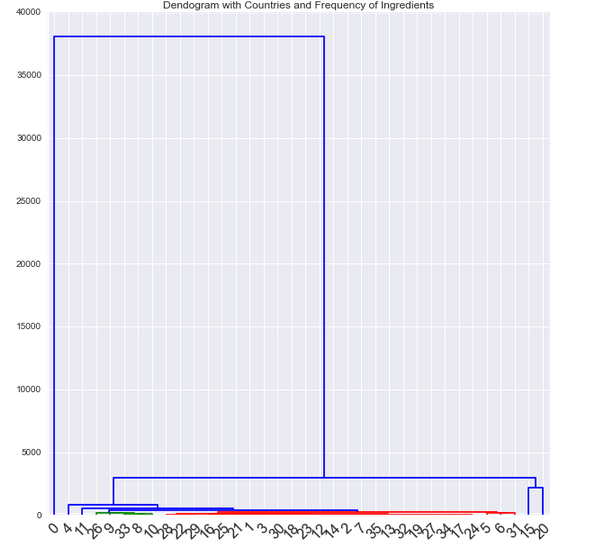
\includegraphics[width=\textwidth]{Countries_Ingredients.png}
\end{minipage}

\raggedright

Here, the 0 corresponds to America. Thus, proof that American recipes differ the most from the rest of the world. 

\vspace{3mm}
\textbf{The disparity is real.} Okay, like me, you're probably curious about this difference a little more. I looked more into the data to find the ingredient that is the most popular in North America and America that separates us from the rest of the world. You ready to hear the result? Eggs. That's right, eggs. In both North America and America, the most popular ingredient is eggs. I created a plot of how many recipes have eggs in them for both the regions and countries and the disparity is real, my reader. 

For the regions, we have this plot:

 \centering
\begin{minipage}[t]{.9\textwidth}
	\includegraphics[width=\textwidth]{Regions_Eggs.png}
\end{minipage}

\raggedright

For the countries, we have this plot:

\centering
\begin{minipage}[t]{.9\textwidth}
	\includegraphics[width=\textwidth]{Countries_Eggs.png}
\end{minipage}

\raggedright

\vspace{5mm}
\textbf{The Numb3rs.} Looking deeper into the numbers, I found that 14,802 North American recipes use eggs and the next highest comes from Western European recipes with only a meager 468 recipes. Furthermore,  14,528 of those North American recipes are American recipes that use eggs. The second runner up for country cuisines that use eggs is Italy with only 411 recipes that use eggs. Conclusion: Americans are crazy about eggs. 

\vspace{5mm}
Welcome to the Englightenment. 

\begin{thebibliography}{}

\bibitem{} Ahn, Yong-Yeol, et al. "Flavor network and the principles of food pairing." Scientific reports 1 (2011).

\bibitem{} Milne, Larissa And Michael. "Travel Reveals 10 Ways America Is Different From the Rest of the World." The Huffington Post. TheHuffingtonPost.com, 26 Jan. 2014. Web. 21 Mar. 2015.

\bibitem{} Milne, Larissa And Michael. "Travel Reveals How America Is Different From the Rest of the World, Part 2." The Huffington Post. TheHuffingtonPost.com, 25 Jun. 2014. Web. 21 Mar. 2015.

\end{thebibliography}

\end{document}